% Created by Bonita Graham
% Last update: December 2019 By Kestutis Bendinskas

% Authors: 
% Please do not make changes to the preamble until after the solid line of %s.

\documentclass[10pt]{article}
\usepackage[explicit]{titlesec}
\setlength{\parindent}{0pt}
\setlength{\parskip}{1em}
\usepackage{hyphenat}
\usepackage{ragged2e}
\RaggedRight

% These commands change the font. If you do not have Garamond on your computer, you will need to install it.
\usepackage{garamondx}
\usepackage[T1]{fontenc}
\usepackage{amsmath, amsthm}
\usepackage{graphicx}
\usepackage{float}

% This adjusts the underline to be in keeping with word processors.
\usepackage{soul}
\setul{.6pt}{.4pt}


% The following sets margins to 1 in. on top and bottom and .75 in on left and right, and remove page numbers.
\usepackage{geometry}
\geometry{vmargin={1in,1in}, hmargin={.75in, .75in}}
\usepackage{fancyhdr}
\pagestyle{fancy}
\pagenumbering{gobble}
\renewcommand{\headrulewidth}{0.0pt}
\renewcommand{\footrulewidth}{0.0pt}

% These Commands create the label style for tables, figures and equations.
\usepackage[labelfont={footnotesize,bf} , textfont=footnotesize]{caption}
\captionsetup{labelformat=simple, labelsep=period}
\newcommand\num{\addtocounter{equation}{1}\tag{\theequation}}
\renewcommand{\theequation}{\arabic{equation}}
\makeatletter
\renewcommand\tagform@[1]{\maketag@@@ {\ignorespaces {\footnotesize{\textbf{Equation}}} #1.\unskip \@@italiccorr }}
\makeatother
\setlength{\intextsep}{10pt}
\setlength{\abovecaptionskip}{2pt}
\setlength{\belowcaptionskip}{-10pt}

\renewcommand{\textfraction}{0.10}
\renewcommand{\topfraction}{0.85}
\renewcommand{\bottomfraction}{0.85}
\renewcommand{\floatpagefraction}{0.90}

% These commands set the paragraph and line spacing
\titleformat{\section}
  {\normalfont}{\thesection}{1em}{\MakeUppercase{\textbf{#1}}}
\titlespacing\section{0pt}{0pt}{-10pt}
\titleformat{\subsection}
  {\normalfont}{\thesubsection}{1em}{\textit{#1}}
\titlespacing\subsection{0pt}{0pt}{-8pt}
\renewcommand{\baselinestretch}{1.15}

% This designs the title display style for the maketitle command
\makeatletter
\newcommand\sixteen{\@setfontsize\sixteen{17pt}{6}}
\renewcommand{\maketitle}{\bgroup\setlength{\parindent}{0pt}
\begin{flushleft}
\sixteen\bfseries \@title
\medskip
\end{flushleft}
\textit{\@author}
\egroup}
\makeatother

% This styles the bibliography and citations.
%\usepackage[biblabel]{cite}
\usepackage[sort&compress]{natbib}
\setlength\bibindent{2em}
\makeatletter
\renewcommand\@biblabel[1]{\textbf{#1.}\hfill}
\makeatother
\renewcommand{\citenumfont}[1]{\textbf{#1}}
\bibpunct{}{}{,~}{s}{,}{,}
\setlength{\bibsep}{0pt plus 0.3ex}




%%%%%%%%%%%%%%%%%%%%%%%%%%%%%%%%%%%%%%%%%%%%%%%%%

% Authors: Add additional packages and new commands here.  

% Limit your use of new commands and special formatting.

% Place your title below. Use Title Capitalization.
\title{Local Network Audit with Nmap}

% Add author information below. Communicating author is indicated by an asterisk, the affiliation is shown by superscripted lower case letter if several affiliations need to be noted.
\author{
Larsen Close*$^{a}$ \\ \medskip 
$^{a}$Computer Science, Metropolitan State University, Denver, CO \\ 
Student: lclose@msudenver.edu \\
}

\pagestyle{empty}
\begin{document}

% Makes the title and author information appear.
\vspace*{.01 in}
\maketitle
\vspace{.12 in}

\section*{abstract}
Extensive Nmap scanning to fingerprint a local network is demonstrated and areas of interest are identified. Anomolies, security concerns
 and unexpected results prompt further investigation. Actions taken upon the basis of the findings are then discussed.


\section*{Motivation}
We often only pay attention to our internet connected devices when we lose connectivity. We then try and restore the connection as quickly
 as possible. The truth is that as the Internet Of Things expands and our world increasingly digitizes the danger of these devices to our 
 safety, privacy and security increases. The steps clearly demonstrated in this paper are steps everyone should take regulary on their home 
 network for their sake and for their families sake.

\vspace{.12 in}

% Start the main part of the manuscript here.
% Comment out section headings if inappropriate to your discipline.
% If you add additional section or subsection headings, use an asterisk * to avoid numbering. 

\section*{introduction}

I started fingerprinting my network with a few areas of heightened interest. In order to ensure a thorough investigation I first used widespread scanning and looked for abnormalties, 
anything which surprised me or that raised security concerns. I made sure to turn on and log into every device on the network before conducting the scans. Also in order to asses the behavior 
of a new automated system for the door lock and thermostat, mandated by the poperty owner, I connected to the network for the first time. The device has been running on cellular connection 
but has both options. 

\subsection*{How does Tails handle local traffic?}

To research the local network scan response of Tails, The Amnesic Incognito Live System (a security-focused Debian based distribution of Linux) I booted a machine 
with the live system during the scans. Starting with cursory scans and increasing the intensity each time while saving the results allowed for a detailed fingerprint of the local network. 

\subsection*{Let shodan.io scan for you}

To gain information about my public IP address and check for any outward facing access I used shodan.io. 
After using their search function I created a monitor with triggers to notify me of any any unexpected activity. After scanning extensively I created the graphs below to organize the findings, visualize them and decide upon which areas to increasingly 
focus. Host data from the scans is combined with DHCP Reservations from the routers to verify the identity of devices and fill gaps left by scans.

\section*{methods and measurement}
To begin scanning we needed to know which IP addresses to tell nmap to scan. Using the command: \begin{verbatim}ifconfig | grep broadcast\end{verbatim} 
We determined the local networks and the subnet ranges. As can be seen in \textbf{Figure \ref{ifconfig image}}, the networks are \verb|10.0.0.0/24|
\verb|192.168.0.0/24|. The \verb|netmask 0xffffff00| tells us the range for hosts is limited the last octet, digits 1-254.

\begin{figure}[H]
\centering
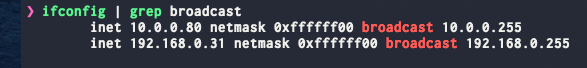
\includegraphics[width=0.5\textwidth]{ifconfig.png}
\caption{First the command 'ifconfig | grep broadcast' identifies the local networks.}\label{ifconfig image}
\end{figure}

\medskip
\subsection*{Super user privileges for scanning}
Next I ran a ping scan of both networks to quickly get a list of the hosts. It's likely that you will not get a full list if you do not run this command with super user privileges.
Testing this without the sudo command resulted in 1 host and 9 hosts respectively. To run ping scans for both networks we used commands:
\begin{verbatim}
sudo nmap -sn 192.168.0.0/24
sudo nmap -sn 10.0.0.0/24 \end{verbatim}
\begin{figure}[H]
\centering
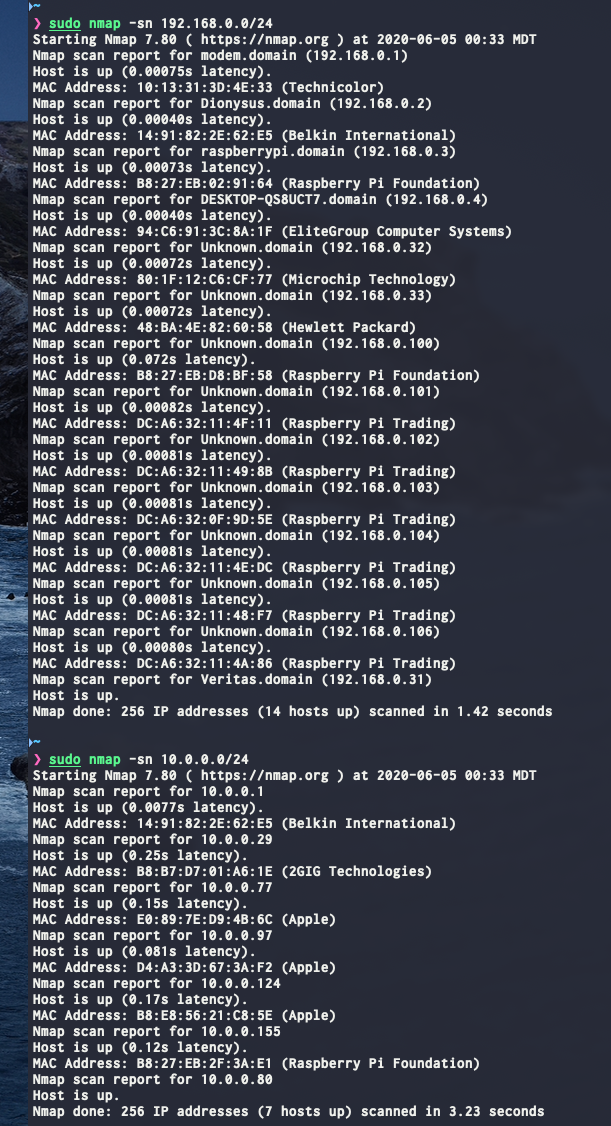
\includegraphics[width=0.5\textwidth]{ping.png}
\caption{A ping scan of both networks returns a list of 14 and 7 hosts.}\label{ping image}
\end{figure}
As we can see in \textbf{Figure \ref{ping image}}, the ping scan with sudo returned a list of 14 hosts and 7 hosts respectively. 

\subsection*{Nmap flags for more thorough scans}
After completing the quick and simple ping scan we scanned both networks using nmap with the flag \verb|-A| to initiate an agressive scan. We also included \verb|-v| to increase the 
verbosity of our results and \verb|-T5| to turn the scans speed all the way up. The commands used here:
\begin{verbatim}
sudo nmap -T5 -A -v 192.168.0.0/24
sudo nmap -T5 -A -v 10.0.0.0/24\end{verbatim}
At this point it was necessary to create \textbf{Table \ref{local table}} to organize the results and create an overview that could actually be visualized. These 
types of scans return so much information that it demands systematic organization. Zenmap can do a good job of helping with this but it has not been running
well for me on macOS Catalina. Another option which I employed is to use an additional flag when running nmap \verb|-oX 'scan-%T-%D.xml'| which outputs the
scan in xml format named by the date and time. To give some full examples:
\begin{verbatim}
sudo nmap -oX 'scan-%T-%D.xml' -T5 -A -v 192.168.0.0/24
sudo nmap -oX 'scan-%T-%D.xml' -T5 -A -v 10.0.0.0/24\end{verbatim}

\subsection*{Checking and monitoring public IP addresses with shodan.io}
Due to the ethical and legal restrictions on scanning the public IP owned by Century Link I used shodan.io to search for my IP and set up a monitor for the address.
An easy what to determine your public IP address is with command:
\begin{verbatim}
curl ifconfig.me
\end{verbatim}

\section*{results}
To begin with, shodan.io allowed us to determine that our router has an open outward facing port. It is running http with authentication. \textbf{Figure \ref{shodan image}} 
shows a screen shot from their webservice.

\begin{figure}[H]
\centering
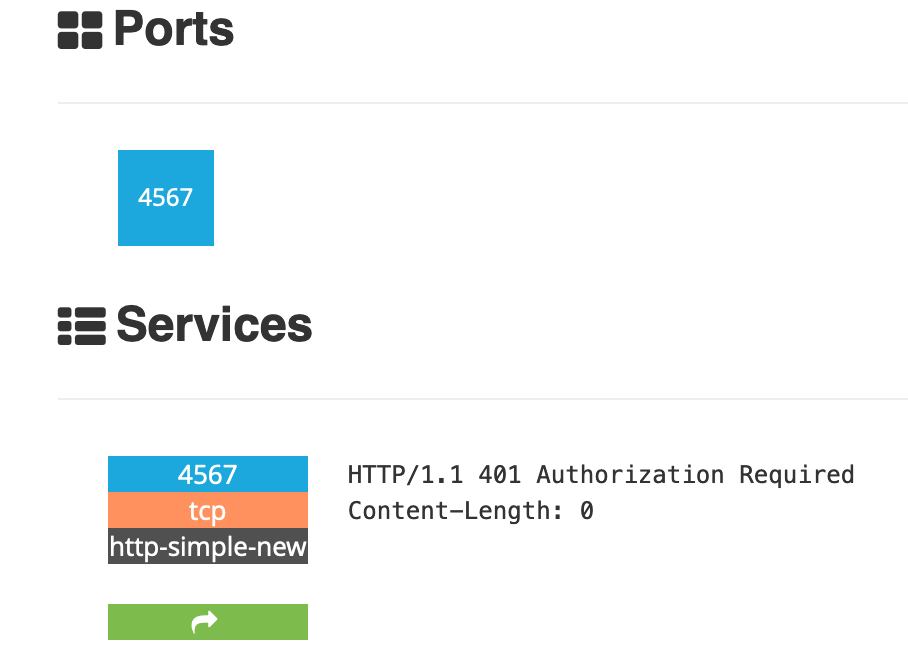
\includegraphics[width=0.5\textwidth]{shodan.png}
\caption{From website https://www.shodan.io/ often called "the most dangerous search engine in the world"}\label{shodan image}
\end{figure}

\subsection*{Compiling all of the findings}
The table below, \textbf{Table \ref{local table}}, is a compilation of all the scans. The aggressive scans discovered more hosts missed by the privileged ping scan.
Immediately some interesting things are visible from the table. First, my HomePod has two IP addresses on the same network. After logging into and checking the router
it appeared that both were running on the 5G wifi. Nmap guessed the 

\begin{table}[H]
  \begin{center}
  \begin{tabular}{ | c | c | c | c | c | c | c | c | } 
  \hline
   & \textbf{Hostname} & \textbf{Device} & \textbf{Purpose} & \textbf{OS} & \textbf{Open} & \textbf{Filtered}  & \textbf{Services}  \\  
   \hline
   \textbf{10.0.0.001} & Dionysus & Router & Gateway & - & 53,80,443,10000 & - & ssl,http \\  
   \hline
   \textbf{10.0.0.029}  & HD100 & Webcam & Security & - & 554,49152 & - & rtsp,UPnP \\  
   \hline
   \textbf{10.0.0.077}  & Daemon & HomePod & Music & audioOS & 62078 & 24 dif & c\\  
   \hline
   \textbf{10.0.0.080}  & Veritas & MacLaptop & PC & macOS & 3000 & c & c \\  
   \hline
   \textbf{10.0.0.097}  & Daemon & HomePod & Music & audioOS & 6 dif & 100 dif & wiretap \\  
   \hline
   \textbf{10.0.0.124}  & Mercury & Watch & Fitness & watchOS & c & 17 dif & wiretap/tracker \\  
   \hline
   \textbf{10.0.0.155}  & raspberrypi & rpi & dev & Buster & 22 & - & ssh \\  
   \hline
   \textbf{}  &  &  &   &  &  &  & \\  
   \hline
   \textbf{192.168.0.001}  & Century Link & Router & Gateway & - & 23,80,433,8085 & - & telnet\\  
   \hline
   \textbf{192.168.0.001}  & Century Link & Outward & Outward & - & 4576 & - & auth http\\  
   \hline
   \textbf{192.168.0.002}  & Dionysus & Router & Secondary & - & All & - & - \\  
   \hline
   \textbf{192.168.0.003}  & raspberrypi & rpi & dev & Buster & 22 & - & ssh \\  
   \hline
   \textbf{192.168.0.004}  & DESKTOP-QS8UCT7 & WindowsPC & PC & Windows & - & All & - \\  
   \hline
   \textbf{192.168.0.031} & Veritas & MacLaptop & PC & macOS & 3000 & - & grafana \\
   \hline
   \textbf{192.168.0.032} & Unknown & ? & 80:1f:12:c6:cf:77 & Linux & 22 & - & ssh \\
   \hline
   \textbf{192.168.0.033} & Unknown & HPLaptop & tails & tails live & - & All & - \\  
   \hline
   \textbf{192.168.0.100}  & Ares & rpi & motion & Buster & 22,3389,8081 & - & xrdp,motion \\  
   \hline
   \textbf{192.168.0.101}  & Master & rpi & Kubernetes & Buster & 22,80,443 & - & - \\  
   \hline
   \textbf{192.168.0.102}  & Node1 & rpi & Kubernetes & Buster & 22,80,443 & - & - \\  
   \hline
   \textbf{192.168.0.103}  & Node2 & rpi & Kubernetes & Buster & 22,80,443 & - & - \\  
   \hline
   \textbf{192.168.0.104}  & Node3 & rpi & Kubernetes & Buster & 22,80,443 & - & - \\  
   \hline
   \textbf{192.168.0.105}  & Node4 & rpi & Kubernetes & Buster & 22,80,443 & - & - \\  
   \hline
   \textbf{192.168.0.106}  & Node5 & rpi & Kubernetes & Buster & 22,80,443 & - & - \\  
   \hline
  \end{tabular}
  \caption{The table itself should be centered.  The table title In AJUR goes below the table and ends with a period. Please bold column and row titles.}
  \label{local table}
  \end{center}
  \end{table}


\section*{conclusions}
Describe major outcomes, novelty, and significance of your work. Future work may be noted.

%There will be no "notes on references" section in your final draft, please remove this section heading.
\section*{notes on references}

Use no indents. Follow the style given in the examples (journals and serial publications;\cite{journal} chapters and monographs;\cite{chapters} web sources,\cite{web} correspondingly) below. All references in text must be in order of appearance. Please include all authors, the complete title, and inclusive pagination, \textit{e.g.}, 1234--1237, not 1234--7; \ul{please make sure to use en-dash} (in \LaTeX, use \verb+--+) \ul{and not the regular dash or em-dash to indicate duration between page numbers or years.} The publication year should follow authors in parentheses. Supply DOI numbers whenever possible. \textit{Book titles} and \textit{web sites} are italicized. \textit{Titles of journals} should be abbreviated according to http://www.abbreviations.com/jas.php. \textbf{\ul{Reference accuracy is critical. It is authors responsibility to carefully check each reference.}} 

In the text, separate superscripted numbers by comma and space,\cite{journal,chapters} they should be separated by an en-dash if the consecutive list of more than two numbers is used.\cite{journal,chapters,web} List them AFTER punctuation (be it comma or period) with no space.

\begin{thebibliography}{9} %If you have more than 9 sources listed, replace this "9" with "99".

\bibitem{journal} Marquez, V., Frohlich, T., Armache, J. P., Sohmen, D., Donhofer, A., Mikolajka, A., Berninghausen, O., Thomm, M., Beckmann, R., Arnold, G. J., and Wilson, D. N. (2011) Proteomic characterization of archaeal ribosomes reveals the presence of novel archaeal-specific ribosomal proteins, \textit{J Mol Biol} 405, 1215--1232. \textit {https://doi.org/10.33697/ajur.2019.003}


\bibitem{chapters} Fierke, C. A., and Hammes, G. G. (1996) Transient Kinetic Approaches to Enzyme Mechanisms, in \textit{Contemporary Enzyme Kinetics and Mechanism} (Purich, D., Ed.) 2nd ed., 1--35, Academic Press, New York.

\bibitem{web} Agricultural Research Service, U.S.D.A. National Nutrient Database for Standard Reference, Release 26, \textit{http://ndb.nal.usda.gov/ndb/search/list} (accessed Mar 2014)
\end{thebibliography}

% The Press Summary section is NOT optional.  Write a paragraph describing the paper in a manner suitable for the press; see previous journal editions for examples.
\section*{reflection}

Please rewrite your abstract so that it captures in few sentences the scope and focus of your publication but could be easily understood by the general public and hopefully shows why your work is exciting and important.

Once done, review these guidelines and the entire document. Make sure that images are exactly where you want them, not at the end of the text. Insert page brakes to avoid orphan titles, words, or sentences being separated out at the end or the top of a page. If any questions remain, please e-mail editor@ajuronline.org.

When you are ready to submit your article, use the share button above and send the read and edit  link.
\end{document}
